\documentclass[8pt,letterpaper]{article}
\usepackage[left=12mm, top=0.5in, bottom=1.5in]{geometry}
\usepackage[utf8]{inputenc}
\usepackage{polski}
\usepackage{amsmath}
\usepackage{multirow}
\usepackage{listing	s}
\usepackage{graphicx}
\usepackage{enumerate}

\begin{document}

\title{Obliczenia naukowe \protect\\  \normalsize Lista druga}

\author{Mateusz Jachniak \protect\\ \normalsize 236738}
\maketitle

\section{Zadanie pierwsze}
  
\subsection{Opis problemu}

\hspace{1.0 cm} Zadanie polegało na zbadaniu wpływu jakie spowodowała niewielka zmiana danych wejściowych z zadania piątym z listy pierwszej.
 
\subsection{Rozwiązanie}
\hspace{1.0 cm} Rozwiązanie jest dokładnie takie same, jak w zadaniu piątym listy pierwszje, jedynie dane wejściowe uległy niewielkiej modyfikacji tzn: $x_4 = 0.5772156649$ na $x'_4=0.577215664$ oraz $x_5 = 0.3010299957$ na $x'_5 = 0.301029995$.

\subsection{Wyniki i interpretacja}

\begin{center}
Tabela z wynikami:
\\
\begin{tabular}{|c|c|c|c|c|}
\hline
\multirow{2}{*}{Algorytm}   & \multicolumn{2}{c|}{Dane oryginalne} & \multicolumn{2}{c|}{Dane zmodyfikowane} \\
                            \cline{2-5}
                            & Float32 & Float64 & Float32 & Float64\\
\hline
\hline
Algorytm 1 & -0.4999443 & 1.0251881368296672e-10 & -0.4999443 & 	-0.004296342739891585\\

Algorytm 2 & -0.4543457 & -1.5643308870494366e-10 & -0.4543457 & -0.004296342998713953\\

Algorytm 3 & -0.5 & 0.0 & -0.5 & -0.004296342842280865\\

Algorytm 4 & -0.5 & 0.0 & -0.5 & -0.004296342842280865\\
\hline

\end{tabular}
\end{center}

\hspace{1.0 cm}Pierwszą obserwacją jest to, że pomimo zmiany danych wejściowych, wyniki działania algorytmów dla arytmetyki Float32 pozostały bez zmian. Z powodu ograniczeń arytmetyki Float32 liczby $x_4$ i $x'_4$ są zapisywane dokładnie tak samo. Reprezentacje bitowe liczb $x_5$ i $x'_5$ różnią się tylko na najmniej znaczącym bicie. Tak mała zmiana wartości danych nie jest możliwa do uchwycenia w arytmetyce \texttt{Float32}, obliczenia były wykonywane na niemal identycznych wartościach, dlatego zakończyły się identycznymi wynikami mimo zmiany danych wejściowych.\\
\hspace*{1.5 cm}W przeciwieństwie do arytmetyki \texttt{Float32}, dla arytmetyki \texttt{Float64} nastąpiły zmiany wyników. Po zmianie danych wyniki nadal znacznie się różnią od prawdziwej wartości, jednak można zauważyć, że dla wszystkich 4 algorytmów uzyskane wyniki są podobne.

\subsection{Wnioski}

\hspace{1.0 cm} Arytmetyka \texttt{Float32} ma na tyle niską precyzję, że bardzo małe zmiany danych wejściowych nie zawsze powodują zmiany wyników. W arytmetyce \texttt{Float64} można zauważyć, że małe zmiany danych mogą być o wiele bardziej widoczne w zmianach wyników obliczeń. Będzie to problemem przy obliczaniu zadań źle uwarunkowanych, tak jak w tym przypadku. l
 

\section{Zadanie drugie}
\subsection{Opis problemu}
\hspace{1.0 cm}W zadaniu należało narysować wykres funkcji $f(x) = e^x ln(1 + e^{-x})$ w co najmniej dwóch programach oraz obliczyć granicę $lim_{x \rightarrow \infty} f(x)$ i porównać wynik z wykresami.


\subsection{Rozwiązanie}
\hspace{1.0 cm} Samodzielnie obliczona wartość granicy: $lim_{x \rightarrow \infty} f(x) = 1$.\\ Do narysowania wykresów wykorzystałem strone internetową: "pl.easima.com" oraz $WolframAlpha$.

\subsection{Wyniki i interpretacja}

\begin{figure}[h!]
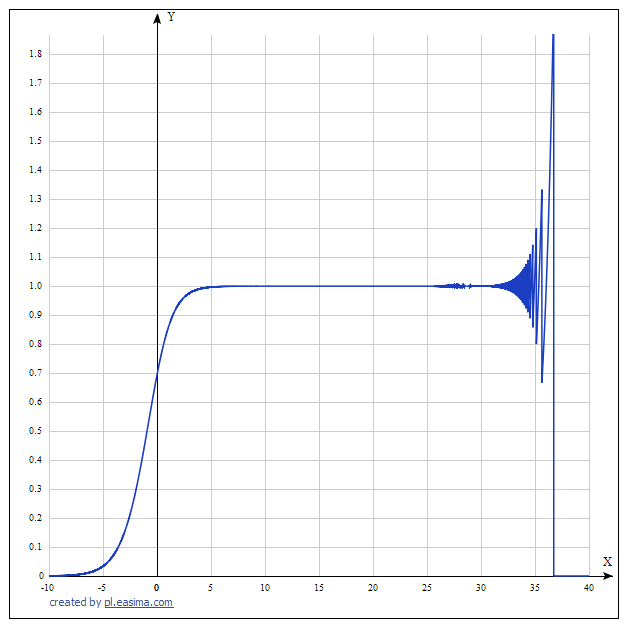
\includegraphics[width=\linewidth]{First_chart.png}
\caption{$f(x)$ w $pl.easima.com$}
\end{figure}

\pagebreak
\hspace{1 cm} Na załączonych wykresach widać, że rzeczywiście dla małych, dodatnich $x$ wykres funkcji zbiega do wartości $1$, jednak wartość funkcji w pewnym momencie gwałtownie spada do $0$ i już się nie zmienia. Wykresy sugerują że granicą tej funkcji jest $0$. Dzieje się tak ponieważ dla dużych $x$ wartość $1 + e ^{-x} = 1$, natomiast $ln(1) = 0$. Dla dużych $x$ otrzymujemy $f(x) = e^xln(1) = e^x*0 = 0$. Dodatkowo, widoczne na wykresach zaburzenia wartości spowodowane są redukcją cyfr znaczących przy dodawaniu $1 + e^{-x}$.

\subsection{Wnioski}
\hspace{1 cm}Często wykorzystujemy do rysowania wykresów funkcji gotowe programy. Należy jednak mieć na uwadzę to, że komputer ma swoje ograniczenia i mimo, że często narysuje wykres szybciej niż człowiek, to może on w pewnym popełnić błąd. Dlatego też nie należy zawsze ufać maszynie, a samemu czasem rozwiązać problem matematyczny, a dopiero później sprawdzić wyniki i zastanowić się, skąd wzięły się różnice.



\section{Zadanie trzecie}
  
\subsection{Opis problemu}

\hspace{1.0 cm} Zadanie polegało na rozwiązaniu układu równań liniowych Ax = b dla A będącego macierzą Hilberta oraz macierzą losową stopnia n o zadanym wskaźniku uwarunkowania. Układy miały być rozwiązane za pomocą dwóch sposobów: eliminacji Gaussa oraz x = $A^{-1}$b.
 
\subsection{Rozwiązanie}
\hspace{1.0 cm}Rozwiązywanie układu równań liniowych zaczynamy od wygenerowania macierzy Hilberta, bądź macierzy losowej przy użyciu odpowiednio funkcji hilb(n) i matcond(n, c) (podanych przez prowadzącego kurs), gdzie n to stopień macierzy, a c zadany wskaźnik uwarunkowania. Następnie tworzymy $x = (1, ..., 1) ^{T}  $ i  $b = (0, ..., 0)^{T} $przy użyciu funkcji ones(n) oraz zeros(n) z języka Julia. Wektor prawych stron otrzymujemy poprzez wykonanie b = A * x. Teraz przystępujemy do rozwiązywania układu równań liniowych. Macierze, na których operujemy muszą być nieosobliwe. Macierz Hilberta jest nieosobliwa (wiemy, że jest kwadratowa, a jej wyznacznik jest różny od 0), ale w przypadku macierzy losowej dodatkowo sprawdzamy czy det(A) $!=$ 0. Układy równań rozwiązujemy poprzez zastosowanie eliminacji Gaussa  oraz x = $A^{-1}$b.

\subsection{Wyniki i interpretacja}
\begin{center}
Macierz Hilberta:
\\

\begin{tabular}{|c|c|c|c|c|}
                       
\hline
n & rank(A) & cound(A) & błąd względy eliminacja Gaussa  & 	błąd względy $A^{-1}b$  \\
\hline
\hline
1 & 1 & 1.0 & 0.0 & 0.0 \\
2 & 2 & 19.28147006790397 & 5.661048867003676e-16 & 1.4043333874306803e-15 \\
3 & 3 & 524.0567775860644 & 8.022593772267726e-15 & 0.0 \\
4 & 4 & 15513.73873892924 & 4.137409622430382e-14 & 0.0 \\
5 & 5 & 476607.25024259434 & 1.6828426299227195e-12 & 3.3544360584359632e-12 \\
6 & 6 & 1.4951058642254665e7 & 2.618913302311624e-10 & 2.0163759404347654e-10 \\
7 & 7 & 4.75367356583129e8 & 1.2606867224171548e-8 & 4.713280397232037e-9 \\
8 & 8 & 1.5257575538060041e10 & 6.124089555723088e-8 & 3.07748390309622e-7 \\
9 & 9 & 4.931537564468762e11 & 3.8751634185032475e-6 & 4.541268303176643e-6 \\
10 & 10 & 1.6024416992541715e13 & 8.67039023709691e-5 & 0.0002501493411824886 \\
11 & 11 & 5.222677939280335e14 & 0.00015827808158590435 & 0.007618304284315809 \\
12 & 11 & 1.7514731907091464e16 & 0.13396208372085344 & 0.258994120804705 \\
13 & 11 & 3.344143497338461e18 & 0.11039701117868264 & 5.331275639426837 \\
14 & 12 & 6.200786263161444e17 & 1.4554087127659643 & 8.71499275104814 \\
15 & 12 & 3.674392953467974e17 & 4.696668350857427 & 7.344641453111494 \\
16 & 12 & 7.865467778431645e17 & 54.15518954564602 & 29.84884207073541 \\
17 & 12 & 1.263684342666052e18 & 13.707236683836307 & 10.516942378369349 \\
18 & 12 & 2.2446309929189128e18 & 9.134134521198485 & 7.575475905055309 \\
19 & 13 & 6.471953976541591e18 & 9.720589712655698 & 12.233761393757726 \\
20 & 13 & 1.3553657908688225e18 & 7.549915039472976 & 22.062697257870493 \\
\hline
\end{tabular}
\end{center}

\hspace{1.0 cm}Macierz Hilberta jest przykładem macierzy bardzo źle uwarunkowanej. Wskaźnik uwarunkowania dla macierzy Hilberta H n wynosi dla cond(H 6 ) = 1.5e7, a dla cond(H 10 ) = 1.5e13. Im większy wskaźnik uwarunkowania tym wyniki stają się mniej wiarygodne. Jak widać w powyższej tabeli, wskaźnik uwarunkowania dla macierzy Hilberta rośnie bardzo szybko, przez co nawet dla niewielkich n rozwiązania stają się niepoprawne. Liczone błędy względne rosną bardzo szybko dla wyników działania obu algorytmów.



\begin{center}
Macierz losowa o zadanym wskaźniku uwarunkowania:
\\

\begin{tabular}{|c|c|c|c|c|}
                       
\hline
n & rank(A) & cound(A) & błąd względy eliminacja Gaussa & 	błąd względy $A^{-1}b$  \\
\hline
\hline
5 & 5 & 1.0 & 2.0471501066083611e-16 & 2.0471501066083611e-16 \\
5 & 5 & 10.0 & 4.124295487574583e-16 & 5.768888059150691e-16 \\
5 & 5 & 1000.0 & 1.1998218802869006e-14 & 2.252543749271376e-14 \\
5 & 5 & 1.0e7 & 1.4616595375180604e-10 & 9.385703304198744e-11 \\
5 & 5 & 1.0e12 & 1.520839842528324e-5 & 1.3754086591583209e-5 \\
5 & 4 & 1.0e16 & 0.1372499989215545 & 0.14523687548277814 \\
10 & 10 & 1.0 & 3.3121136700345433e-16 & 2.9582808634907537e-16 \\
10 & 10 & 10.0 & 2.1065000811460205e-16 & 1.4043333874306804e-16 \\
10 & 10 & 1000.0 & 1.608360289126608e-14 & 1.9115448498488666e-14 \\
10 & 10 & 1.0e7 & 2.37843535343169e-10 & 2.1866643517582951e-10 \\
10 & 10 & 1.0e12 & 1.5740419510840757e-5 & 1.3200726679228422e-5 \\
10 & 9 & 1.0e16 & 0.1805921046121644 & 0.20610790559801434 \\
20 & 20 & 1.0 & 3.773125249565729e-16 & 4.385029596794321e-16 \\
20 & 20 & 10.0 & 6.176473131037029e-16 & 6.454588798442909e-16 \\
20 & 20 & 1000.0 & 9.16169466901524e-15 & 6.598872780119333e-15 \\
20 & 20 & 1.0e7 & 2.9606040897065132e-12 & 5.5028563368800784e-11 \\
20 & 20 & 1.0e12 & 1.7623490988034295e-5 & 1.6239088298887365e-5 \\
20 & 19 & 1.0e16 & 6.964382220947393e-16 & 0.031213357423395274 \\
\hline
\end{tabular}
\end{center}


\hspace{1.0 cm} Macierz losowa o zadanym wskaźniku uwarunkowania potwierdza obserwacje zależności między wskaźnikiem uwarunkowania a błędem względnym z macierzy Hilberta. Można tutaj dokładnie obejrzeć wpływ wzrastającego, kontrolowanego wskaźnika uwarunkowania na generowane błędy względne. Wraz ze zwiększeniem cond(A) rosną błędy względne algorytmów rozwiązywania układu równań liniowych dla macierzy o zadanym n.

\subsection{Wnioski}

\hspace{1.0 cm} Macierze o wysokim wskaźniku uwarunkowania generują duże błędy w obliczeniach. Pojawienie się macierzy Hilberta podczas obliczeń może sprawić, że otrzymane wyniki będą niewiarygodne. Na szczególną uwagę zasługuje stopień „złośliwości” macierzy Hilberta. Dlatego też numerycznie rozwiązywanie nawet niewielkich układów równań z tą macierzą jest zatem praktycznie niemożliwe, przynajmniej na dzisiejsze czasy.




\section{Zadanie czwarte}
  
\subsection{Opis problemu}

\hspace{1.0 cm} Tutaj treść zadania
 
\subsection{Rozwiązanie}
\hspace{1.0 cm}Badanie zachowania pierwiastków wielomianu Wilkinsona zaczynamy od stworzenia postaci naturalnej wielomianu w języku Julia. Współczynniki wielomianu przechowujemy w tablicy. Wielomian Wilkinsona w postaci naturalnej tworzymy poprzez użycie konstruktora Poly z pakietu Polynomials. Postać iloczynową tworzymy przy użyciu funkcji poly. Ważne jest, aby przekazywane do metod poly oraz Poly współczynniki były uporządkowane od współczynników stojących przy najniższych potęgach x. Pierwiastki wielomianu wyliczamy przy użyciu funkcji roots, a wartość wielomianu dla danego argumentu x za pomocą metody polyval.

\subsection{Wyniki i interpretacja}
W poniższej tabeli przez z k zostały oznaczone wyliczone pierwiastki wielomianu, a przez k dokładne
pierwiastki.
\begin{center}
\begin{tabular}{|c|c|c|c|}
                       
\hline
1 & 2 & 3 & 4  \\
\hline
\hline
0.9999999999996989 & 36352.0 & 38400.0 & 3.0109248427834245e-13 \\
2.0000000000283182 & 181760.0 & 198144.0 & 2.8318236644508943e-11 \\
2.9999999995920965 & 209408.0 & 301568.0 & 4.0790348876384996e-10 \\
3.9999999837375317 & 3.106816e6 & 2.844672e6 & 1.626246826091915e-8 \\
5.000000665769791 & 2.4114688e7 & 2.3346688e7 & 6.657697912970661e-7 \\
5.999989245824773 & 1.20152064e8 & 1.1882496e8 & 1.0754175226779239e-5 \\
7.000102002793008 & 4.80398336e8 & 4.78290944e8 & 0.00010200279300764947 \\
7.999355829607762 & 1.682691072e9 & 1.67849728e9 & 0.0006441703922384079 \\
9.002915294362053 & 4.465326592e9 & 4.457859584e9 & 0.002915294362052734 \\
9.990413042481725 & 1.2707126784e10 & 1.2696907264e10 & 0.009586957518274986 \\
11.025022932909318 & 3.5759895552e10 & 3.5743469056e10 & 0.025022932909317674 \\
11.953283253846857 & 7.216771584e10 & 7.2146650624e10 & 0.04671674615314281 \\
13.07431403244734 & 2.15723629056e11 & 2.15696330752e11 & 0.07431403244734014 \\
13.914755591802127 & 3.65383250944e11 & 3.653447936e11 & 0.08524440819787316 \\
15.075493799699476 & 6.13987753472e11 & 6.13938415616e11 & 0.07549379969947623 \\
15.946286716607972 & 1.555027751936e12 & 1.554961097216e12 & 0.05371328339202819 \\
17.025427146237412 & 3.777623778304e12 & 3.777532946944e12 & 0.025427146237412046 \\
17.99092135271648 & 7.199554861056e12 & 7.1994474752e12 & 0.009078647283519814 \\
19.00190981829944 & 1.0278376162816e13 & 1.0278235656704e13 & 0.0019098182994383706 \\
19.999809291236637 & 2.7462952745472e13 & 2.7462788907008e13 & 0.00019070876336257925 \\
\hline
\end{tabular}
\end{center}

\hspace{1.0 cm}Powyższa tabela przedstawia wyniki dla wielomianu Wilkinsona o niezaburzonych współczynnikach.
Można zauważyć, że wartości wielomianów w postaci naturalnej i iloczynowej różnią się dla pewnych
z k . Widoczna jest również różnica między pierwiastkami wyliczonymi, a rzeczywistymi. Wielomian
Wilkinsona jest bardzo czuły na odchylenia na poziomie przekazywanych argumentów. Oczekiwanymi
wartościami P (z k ) oraz p(z k ) były zera, natomiast otrzymane wyniki znacznie odbiegają od zera. Dla z k kolo 20 jest to odchylenie nawet o 2.74e13. Zauważyć można także, że nawet stosunkowo niewielkie odchylenia danych wejściowych (dla z k kolo 1 błąd jest na poziomie 13 miejsc po przecinku, co widać w kolumnie aaa) potrafią znacznie wpłynąć na wynik końcowy.

\begin{center}
\begin{tabular}{|c|c|c|c|}
                       
\hline
1 & 2 & 3 & 4  \\
\hline
\hline
0.9999999999998357 + 0.0im & 20992.0 & 22016.0 & 1.6431300764452317e-13 \\
2.0000000000550373 + 0.0im & 349184.0 & 365568.0 & 5.503730804434781e-11 \\
2.99999999660342 + 0.0im & 2.221568e6 & 2.295296e6 & 3.3965799062229962e-9 \\
4.000000089724362 + 0.0im & 1.046784e7 & 1.0729984e7 & 8.972436216225788e-8 \\
4.99999857388791 + 0.0im & 4.2535936e7 & 4.3303936e7 & 1.4261120897529622e-6 \\
6.000020476673031 + 0.0im & 2.04793344e8 & 2.06120448e8 & 2.0476673030955794e-5 \\
6.99960207042242 + 0.0im & 1.754868736e9 & 1.757670912e9 & 0.00039792957757978087 \\
8.007772029099446 + 0.0im & 1.852128e10 & 1.8525486592e10 & 0.007772029099445632 \\
8.915816367932559 + 0.0im & 1.37168464896e11 & 1.37174317056e11 & 0.0841836320674414 \\
10.095455630535774 - 0.6449328236240688im & 1.4912572850824043e12 & 1.4912633816754019e12 & 0.6519586830380406 \\
10.095455630535774 + 0.6449328236240688im & 1.4912572850824043e12 & 1.4912633816754019e12 & 1.1109180272716561 \\
11.793890586174369 - 1.6524771364075785im & 3.2960224849741504e13 & 3.2960214141301664e13 & 1.665281290598479 \\
11.793890586174369 + 1.6524771364075785im & 3.2960224849741504e13 & 3.2960214141301664e13 & 2.045820276678428 \\
13.992406684487216 - 2.5188244257108443im & 9.545941965367332e14 & 9.545941595183662e14 & 2.5188358711909045 \\
13.992406684487216 + 2.5188244257108443im & 9.545941965367332e14 & 9.545941595183662e14 & 2.7128805312847097 \\
16.73074487979267 - 2.812624896721978im & 2.7420894080997828e16 & 2.7420894016764064e16 & 2.9060018735375106 \\
16.73074487979267 + 2.812624896721978im & 2.7420894080997828e16 & 2.7420894016764064e16 & 2.825483521349608 \\
19.5024423688181 - 1.940331978642903im & 4.252502487879955e17 & 4.2525024879934694e17 & 2.454021446312976 \\
19.5024423688181 + 1.940331978642903im & 4.252502487879955e17 & 4.2525024879934694e17 & 2.004329444309949 \\
20.84691021519479 + 0.0im & 1.3743733195398482e18 & 1.3743733197249713e18 & 0.8469102151947894 \\
\hline

\end{tabular}
\end{center}

\subsection{Wnioski}

\hspace{1.0 cm} Problem wyznaczania pierwiastków wielomianu Wilkinsona jest źle uwarunkowany ze względu na zaburzenia współczynników. Nawet niewielkie odchylenia danych wejściowych potrafią całkowicie zaburzyć wyniki, co sprawia, że obliczenia na takim wielomianie są niewykonywalne. Naprawdę zasługuje na miano "złośliwego wielomianu".




\section{Zadanie piąte}
\subsection{Opis problemu}
\hspace{1.0 cm}Zadanie polega na symulacji procesu  logistycznego wzrostu populacji. Polecenie trzeba wykonać na 3 sposoby - dla zadanych parametrów przeprowadzić symulację dla typów Float32 i Float64 oraz zmodyfikowaną wersję procesu dla typu Float32. Modyfikacja polega na wykonaniu 10 iteracji zgodnie z rekurencyjnym wzorem, zaokrągleniu otrzymanego wyniku do trzech miejsc po przecinku i przyjąć otrzymany wynik jako argument kolejnego rekurencyjnego wywołania funkcji.
\\
\subsection{Rozwiązanie}
\hspace{1.0 cm}Do przeprowadzenia symulacji użyte zostało podane w opisie problemu wyrażenie. Kolejne wartości wyrażenia, począwszy od p 0 = 0.01 i r = 3 były wyliczane iteracyjnie, a wartości p n były zapisywane w tablicy. Tablica ta służyła potem do odtworzenia kolejnych wartości wyrażenia. Obcięcie wyniku po 10 iteracjach w pierwszej części zadania zostało wykonane przy użyciu funkcji bibliotecznej trunc z języka Julia.

\subsection{Wyniki i interpretacja}

\begin{center}
Tabela z wynikami:
\\
\begin{tabular}{|c|c|c|c|}
\hline

	n&	Float32 & Float32(zmodyfikowany) & Float64 \\
	\hline
	\hline
	1 & 0.0397 & 0.0397 & 0.0397 \\
2 & 0.15407173 & 0.15407173 & 0.15407173000000002 \\
3 & 0.5450726 & 0.5450726 & 0.5450726260444213 \\
4 & 1.2889781 & 1.2889781 & 1.2889780011888006 \\
5 & 0.1715188 & 0.1715188 & 0.17151914210917552 \\
6 & 0.5978191 & 0.5978191 & 0.5978201201070994 \\
7 & 1.3191134 & 1.3191134 & 1.3191137924137974 \\
8 & 0.056273222 & 0.056273222 & 0.056271577646256565 \\
9 & 0.21559286 & 0.21559286 & 0.21558683923263022 \\
10 & 0.7229306 & 0.722 & 0.722914301179573 \\
11 & 1.3238364 & 1.3241479 & 1.3238419441684408 \\
12 & 0.037716985 & 0.036488414 & 0.03769529725473175 \\
13 & 0.14660022 & 0.14195944 & 0.14651838271355924 \\
14 & 0.521926 & 0.50738037 & 0.521670621435246 \\
15 & 1.2704837 & 1.2572169 & 1.2702617739350768 \\
16 & 0.2395482 & 0.28708452 & 0.24035217277824272 \\
17 & 0.7860428 & 0.9010855 & 0.7881011902353041 \\
18 & 1.2905813 & 1.1684768 & 1.2890943027903075 \\
19 & 0.16552472 & 0.577893 & 0.17108484670194324 \\
20 & 0.5799036 & 1.3096911 & 0.5965293124946907 \\
21 & 1.3107498 & 0.09289217 & 1.3185755879825978 \\
22 & 0.088804245 & 0.34568182 & 0.058377608259430724 \\
23 & 0.3315584 & 1.0242395 & 0.22328659759944824 \\
24 & 0.9964407 & 0.94975823 & 0.7435756763951792 \\
25 & 1.0070806 & 1.0929108 & 1.315588346001072 \\
26 & 0.9856885 & 0.7882812 & 0.07003529560277899 \\
27 & 1.0280086 & 1.2889631 & 0.26542635452061003 \\
28 & 0.9416294 & 0.17157483 & 0.8503519690601384 \\
29 & 1.1065198 & 0.59798557 & 1.2321124623871897 \\
30 & 0.7529209 & 1.3191822 & 0.37414648963928676 \\
31 & 1.3110139 & 0.05600393 & 1.0766291714289444 \\
32 & 0.0877831 & 0.21460639 & 0.8291255674004515 \\
33 & 0.3280148 & 0.7202578 & 1.2541546500504441 \\
34 & 0.9892781 & 1.3247173 & 0.29790694147232066 \\
35 & 1.021099 & 0.034241438 & 0.9253821285571046 \\
36 & 0.95646656 & 0.13344833 & 1.1325322626697856 \\
37 & 1.0813814 & 0.48036796 & 0.6822410727153098 \\
38 & 0.81736827 & 1.2292118 & 1.3326056469620293 \\
39 & 1.2652004 & 0.3839622 & 0.0029091569028512065 \\
40 & 0.25860548 & 1.093568 & 0.011611238029748606 \\
	\hline

\end{tabular}
\end{center}

\hspace{1.0 cm} W podpunkcie pierwszym zgodnie z treścią zadania porównuję kolumnę Float32 z Float32(modyfikacja). Od iteracji nr 10 (do której oba przypadki są równe) przez kilka pierwszych iteracji wyniki są dość podobne. Ogromna zmiana następuje w iteracji 20 - wynik jedną metoda to ok, 0.58, a drugą 1.31. Ta róznica sprawia, że od tego momentu wyniki w obu kolumnach są bardzo różne i nie widać żadnej zależności między nimi (jedne rosną, gdy inne maleją itp.)

\hspace{1.0 cm} W podpunkcie drugim zadania dobrze widoczny jest moment, w którym iteracje dla arytmetyki Float32 i Float64 zaczynają dawać różne rezultaty. Dzieje się tak w okolicach 22. iteracji, kiedy dokładność arytmetyki potrzebna na zapisanie wyników wyrażenia rekurencyjnego staje się niewystarczająca, przez co propagacja błędów daje dla tych dwóch iteracji zupełnie nieskorelowane wyniki. Niższa precyzja arymetyki single spowodowała znacznie szybszą akumulację błędu.

\subsection{Wnioski}

\hspace{1.0 cm}Przyczyną odmiennego zachowania wyników w każdej sytuacji jest fakt, że odwzorowanie logistyczne jest układem chaotycznym tzn. małe zmiany warunków początkowych powodują duże zmiany wyników. Oznacza to, że przy badaniu zależności opisanych równianiem jak w treści zadania konieczna jest wyjątkowa dokładnośc ustalenia warunków początkowych. Sposobem chwilowego opóźnienia zbyt dużej akumulacji błędu jest podwyższenie precyzji arytmetyki, jednak nie jest to rozwiązanie wystarczające, gdyż lpropagowany błąd spowoduje występowanie niepoprawnych wyników w dalszych stadiach procesu.

\section{Zadanie szóste}
\subsection{Opis problemu}
\hspace{1.0 cm}Zadanie polega na zbadaniu zachowania równania rekurencyjnego:
\begin{center}
$x_{n+1} = x_{n}^{2}+c$ dla n=0,1,$\dots$
\end{center}
dla następujących danych:

\begin{enumerate}
\item c= -2 i $x_{0}$ = 1
\item c= -2 i $x_{0}$ = 2
\item c= -2 i $x_{0}$ = 1.99999999999999
\item c= -1 i $x_{0}$ = 1
\item c= -1 i $x_{0}$ = -1
\item c= -1 i $x_{0}$ = 0.75
\item c= -1 i $x_{0}$ = 0.25
\end{enumerate}



\subsection{Rozwiązanie}
\hspace{1.0 cm}Aby rozwiązać zadanie wykorzystaliśmy pakiet "Plots" w Julii, aby graficznie przedstawić wyniki dla 40 iteracji dla wyżej przedstawionych danych.

\subsection{Wyniki i interpretacja}

\hspace{1 cm} Dla zadanych danych wejściowych eksperymentów można zaobserwować dwa zjawiska: stabilizacji układu sprzężenia zwrotnego oraz niestabilności związanej ze sprzężeniem zwrotnym.
\begin{figure}[h!]
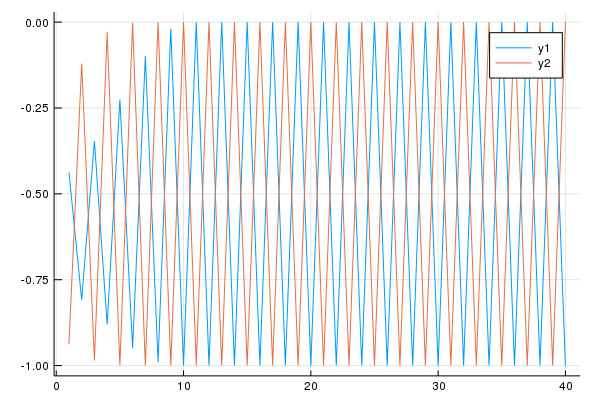
\includegraphics[width=\linewidth]{const_minus_one_second.png}
\caption{Wykres przedstawia przypadek 6 (niebieski) i 7 (pomarańczowy)}
\end{figure}
\hspace{1 cm} W powyższym przypadku, obserwujemy stabilizacje układu sprężenia, jednak następuje ono, dopiero od pewnego momentu (około 10 iteracji).
\begin{figure}[h!]
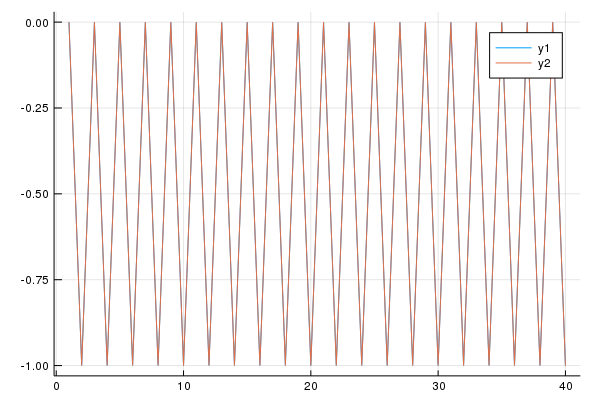
\includegraphics[width=\linewidth]{const_minus_one_first.png}
\caption{Wykres przedstawia przypadek 4 i 5 (są one identyczne, ponieważ $-1^{2} = 1^{2}$)}
\end{figure}

\hspace{1 cm} W tym przykładzie od początku możemy zauważyc stabilizacje układu stężenia.
\begin{figure}[h!]
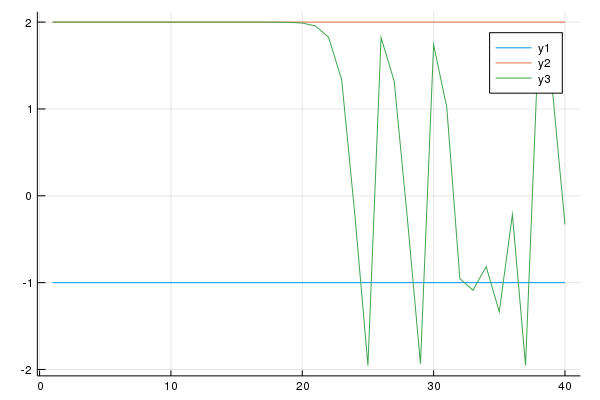
\includegraphics[width=\linewidth]{const_minus_two.png}
\caption{Wykres przedstawia podpunkty 1(niebieski), 2 (pomarańczowy) oraz 3 (zielony)}
\end{figure}

\hspace{1 cm} Przypadki 1 i 2, zachowują się podobnie jak powyżysze, jednak ciekawsza sytuacja kreauje się w trzecim podpunkcie. DODAJ JAKIS MADRY OPIS

\subsection{Wnioski}
\hspace{1 cm}Problem ten pozwolił na zaobserwowanie dwóch zachowań układów sprzężenia zwrotnego: stabilizacji oraz niestabilności. Stabilizację można było zaobserwować jako powtarzanie się przewidywalnych wyników, zaś niestabilność jako generowanie błędnych wyników, spowodowane niewielkimi błędami popełnionymi w początkowych stadiach obliczania wartości wyrażenia. Podobnie jak w zadaniu 5 wprowadzona niestabilność jest skutkiem precyzji arytmetyki double, która była używana do przeprowadzanych w zadaniu obliczeń. Liczba miejsc po przecinku, potrzebnych do przedstawienia kolejnych wyników, zwiększała się, co uniemożliwiało otrzymanie poprawnych wyników.


\end{document}